\section{Introduction}
\label{sec:intro}
Electron micrographs are obtained by cryo-electron tomography (CET) \cite{Hawkes2007} (Figure~\ref{fig:img} (a)), which is an advanced technique to visualize the near-to-native environment of neurones, such as cytosol or lysate and lipid membranes \cite{Lucic2005a}).
Among all kinds of cellular material, biological macromolecules in synaptic cleft regions are one of the hot studying areas, as they play an important role in neurotransmitter transmission.
However in the last ten years, it still depends manual segmentation of synaptic cleft region to analyze those macromolecules of interest, which is time-consuming and subjective.
In this paper, we propose an automatical model using deep convolutional network and a novel contour growing algorithm to segmenting the accurate region of synaptic cleft (Figure~\ref{fig:img} (2)).

However, the challenges behind this tasks are not easy to resolve by existing segmenting methods.
Firstly, due to the radiation damaging during CET, electron micrographs suffers from high noise and low signal-to-noise ratio (SNR).
Secondly, the synaptic cleft region is only a small fraction of a $2D$ electron micrograph of thousands of resolution, which require the model to well segment small objects.
Thirdly, only the cellular clefts, adjacent to one synapse and receives neurotransmitter molecules from another synapse, are our plausible synaptic cleft, which require the model to learn munch biological knowledge for judgement.
Finally, as the most of concerned macromolecules exist on the surface of presynaptic membrane, it puts a high demand on contour localization for the model.

\begin{figure}[t]
    \begin{center}
        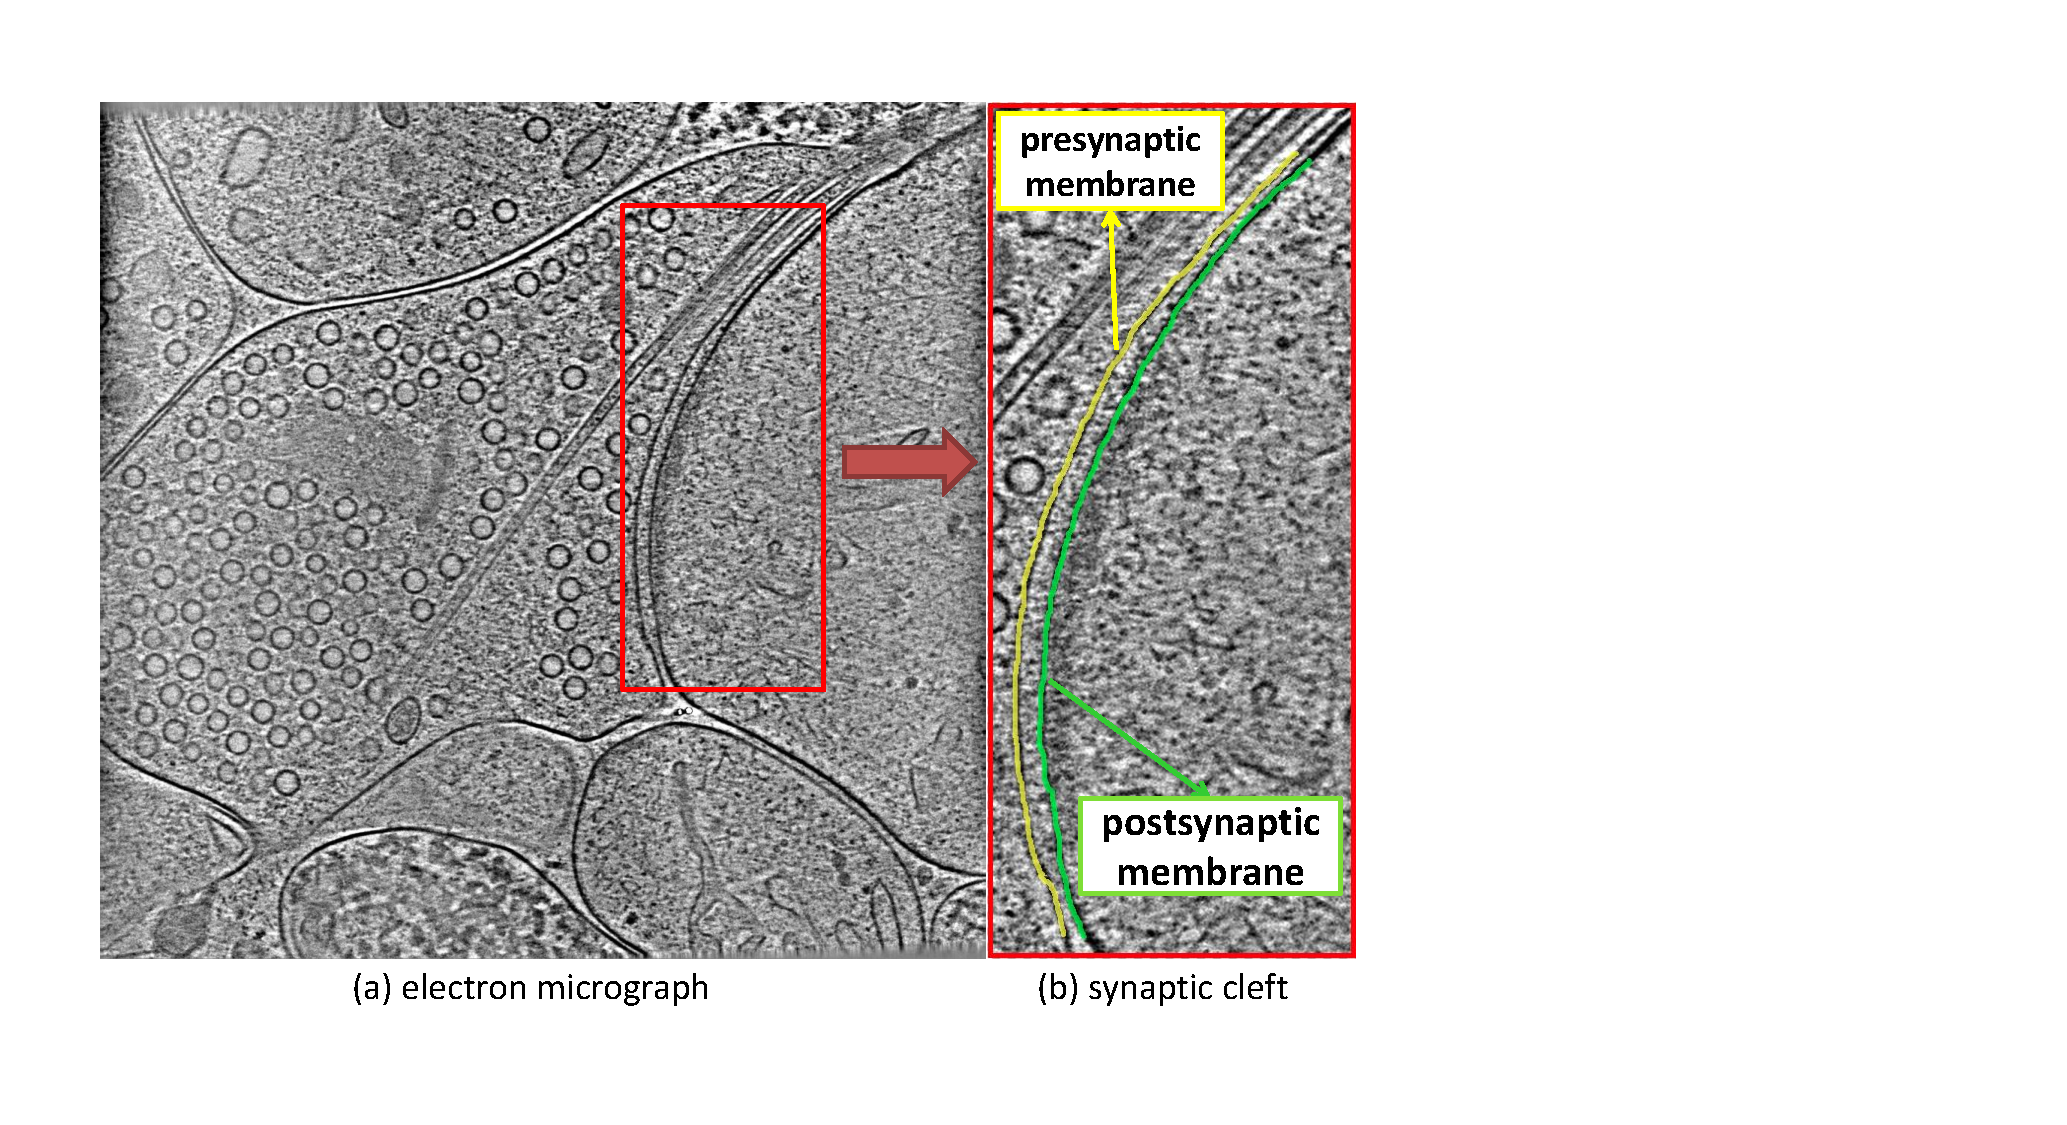
\includegraphics[width=3.4in]{figs/FigImg.pdf}
   \end{center}
\caption{(a) An example of electron micrograph. The red rectangle indicates the synaptic cleft region. 
            (b) Synaptic cleft region corresponding to red rectangle in (a). Especially, the synaptic cleft region is surrounded by presynaptic membrane (yellow curve) and postsynaptic membrane (green curve). }
\label{fig:img}
\end{figure}
Recently, fully convolutional networks (FCN) \cite{Long2015,Ronneberger2015,Chen2016a,Chen2017,Zhao2016} have achieved great progress in image segmentation filed, and variants of FCN \cite{Ronneberger2015,Chen2017,Dhungel2015,Lieman-Sifry2017,Chen2016b,Ourselin} give their promising performance in biomedical image processing.
For examples, the famous U-net \cite{Ronneberger2015} proposed a U-shaped network by directly concatenating the features from downsampling to upsampling layers for supplementing low-level information and better contour localization.
Soon, \cite{Chen2016a} develop the dilated convolution operation by introducing zero into original convolutional kernel for lager perception field and achieve amazing performance in natural image segmentation.
DCAN \cite{Chen2017} integrates complementary information of objects and contours in a multi-task learning framework to separate the clustered objects into individual ones.
And PSPNet \cite{Zhao2016} use the more powerful ResNet \cite{He2016} for feature extracting and propose a pyramid pooling module to for better exploit the global context information.
Although the existing methods have achieved great success in many challenging dataset, they may still fail in processing the electron micrographs, which are much different in texture and information.

\begin{figure*}[t]
    \begin{center}
        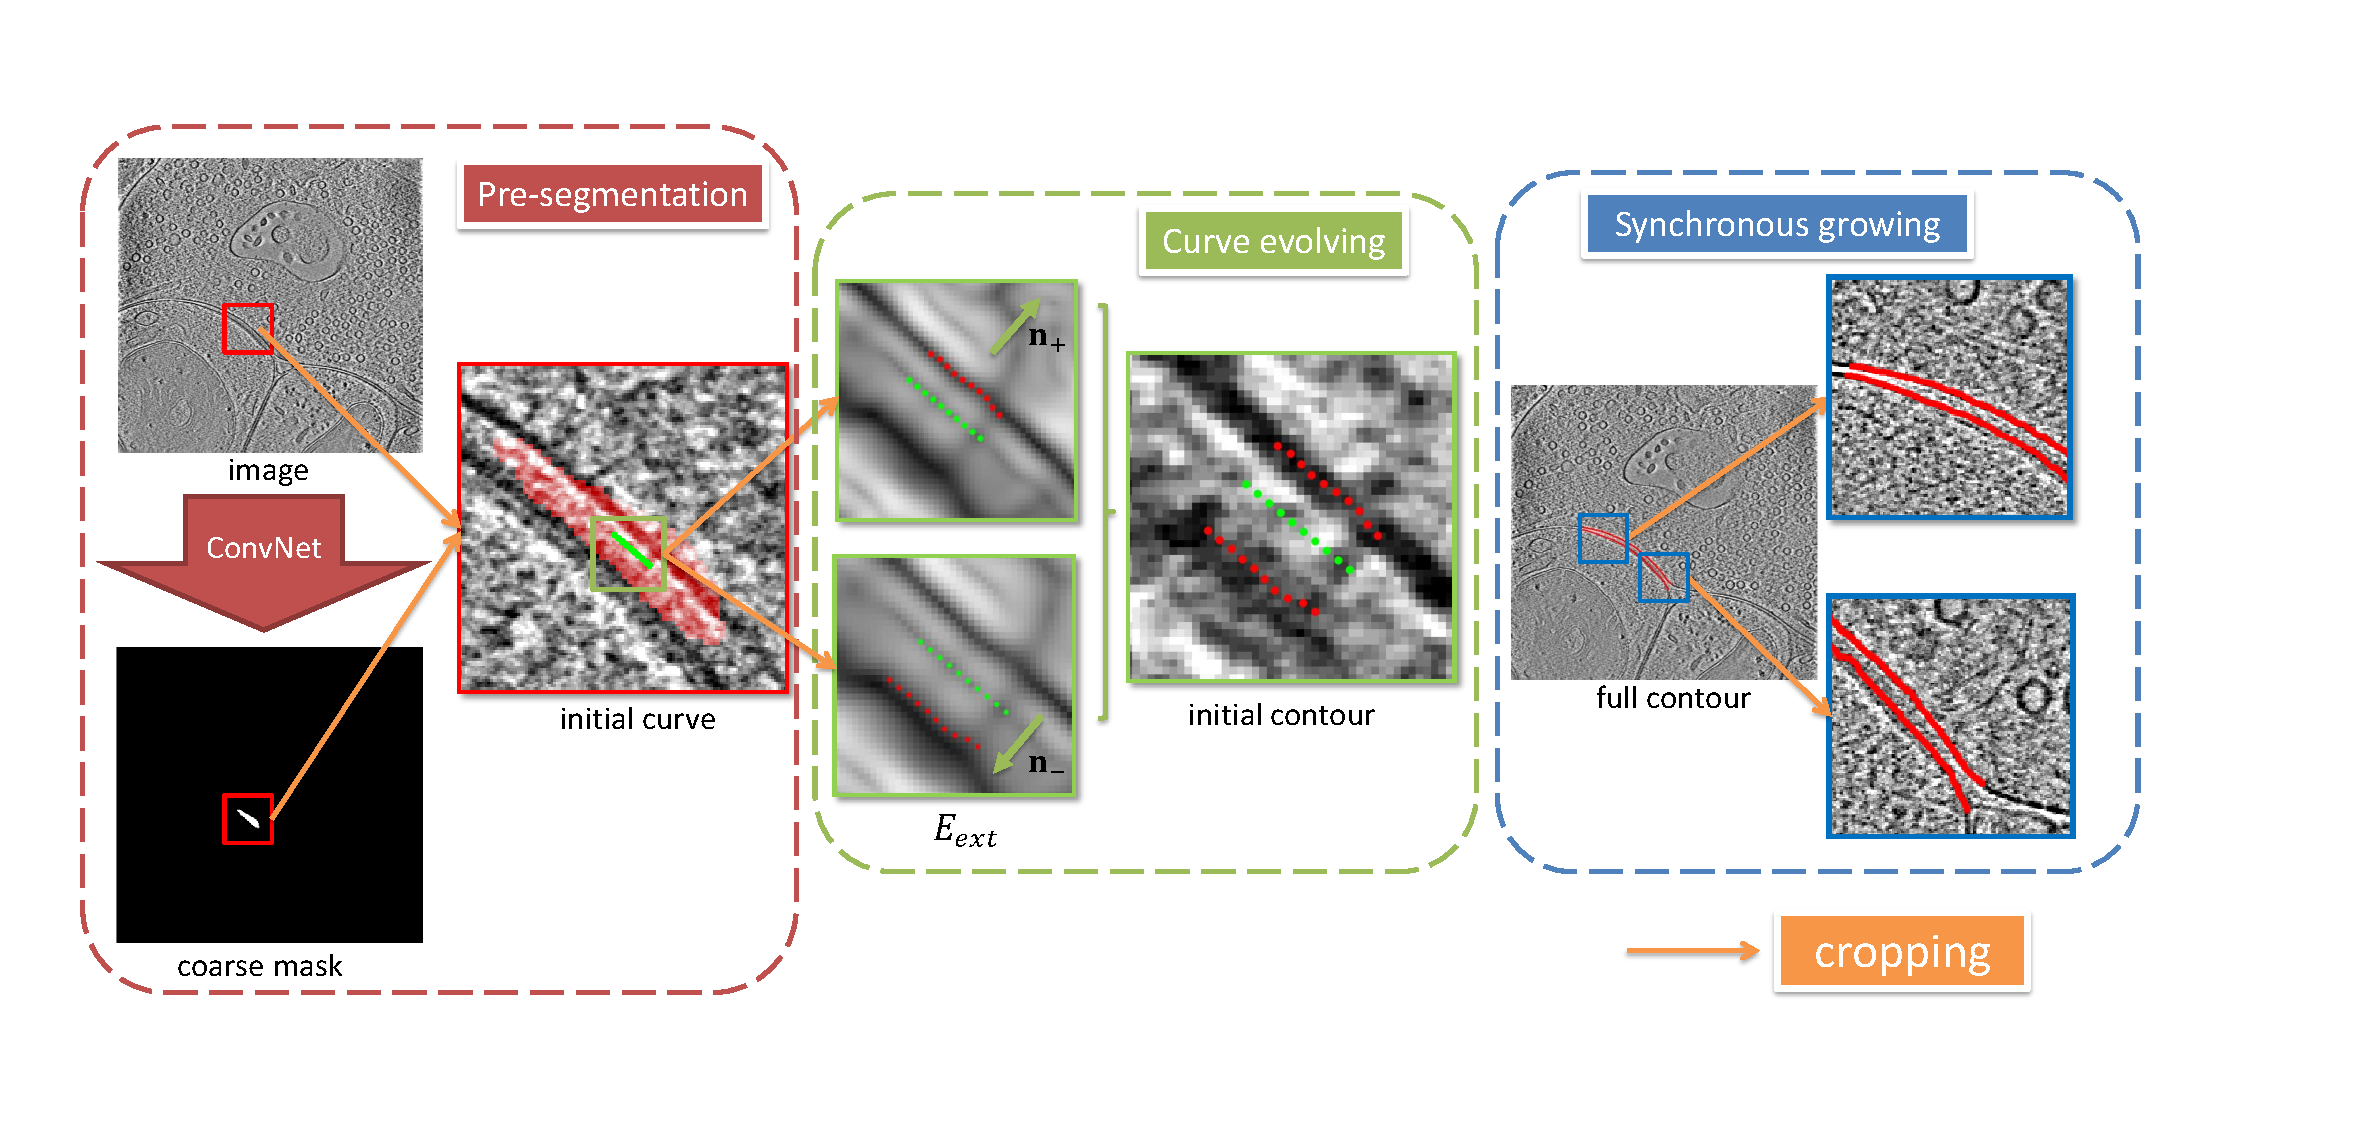
\includegraphics[width=7in]{figs/FigCG.pdf}
   \end{center}
\caption{A brief view of our model in localizing the synaptic cleft region. First a CNN based model results in a coarse segmentation mask, which provides an initial curve (green line) in cleft region.
        Then, the initial curve is respectively evolved along opposite direction ($\mathbf{n}_+$ and $\mathbf{n}_-$) to obtain two piece of initial contours (red dotted line).
        Finally, we will synchronously grow the contours to localize the whole synaptic cleft region (encircled by red solid curves).}
\label{fig:cg}
\end{figure*}
In this paper, we propose an effective framework for segmenting target region in electron micrographs by combining intelligent CNN and a novel contour growing algorithm.
Our method is divided into two steps.
First, a FCN based segmentation is implemented to generate a coarse segmentation of synaptic cleft region.
And then, our contour growing algorithm takes in the segmentation and results in precise contour localizations of target synaptic cleft region.
The insight of our method is that the contours localized by FCNs are usually poor and unsatisfied, due to successive downsampling layers\cite{Chen2017}, but it successfully produce an accurate localization of our plausible region.
Therefore, we utilize the ability of FCN of learning high-level biological knowledge to globally pick out synaptic cleft from such a complex environment, which can be competent for most FCNs.

Our contour growing algorithm is robust and efficient, because it is a self-correcting model and use the local texture information for inference.
With a coarse segmentation of target region, the method first generates a piece of accurate contour from the mask as origin and then gradually grows the whole contours of the target region.
Especially, as long as the major part of initial curve is successfully evolved to target contour, the following growing process will be not affected.
However, since the contour of a synaptic cleft is not closed and consists of the presynaptic and postsynaptic membranes as shown in Figure, we should simultaneously growing two piece of contours and decide when to terminate the growing according to the distance between these two membranes.

Our main contributions are threefold:
\begin{enumerate}
	\item We propose a new framework to accurately segment the target region in electron micrographs.
	\item A novel updating strategy of active contour method is developed, which is more robust and effective.
	\item Specific to segment synaptic cleft region, we propose a algorithm to synchronously grow both two contours.
\end{enumerate}